\xiti
\begin{xiaotis}
\begin{enhancedline}

\xiaoti{已知:如图, $AB \pingxing A'B'$,$BC \pingxing B'C'$。
    求证: $\triangle ABC \xiangsi \triangle A'B'C'$。
}

\begin{figure}[htbp]
    \centering
    \begin{minipage}[b]{7cm}
        \centering
        \begin{tikzpicture}
    \tkzDefPoints{0/0/O, 3/0/C, 4/1.5/B, 2/2.5/A}
    \tkzDefPointOnLine[pos=0.5](O,A)  \tkzGetPoint{A'}
    \tkzDefLine[parallel=through A'](A,B)  \tkzGetPoint{b'}
    \tkzInterLL(A',b')(O,B)  \tkzGetPoint{B'}
    \tkzDefLine[parallel=through B'](B,C)  \tkzGetPoint{c'}
    \tkzInterLL(B',c')(O,C)  \tkzGetPoint{C'}

    \tkzDrawPolygon(O,A,B,C)
    \tkzDrawSegments(O,B  A,C)
    \tkzDrawPolygon(A',B',C')
    \tkzLabelPoints[above](A,B')
    \tkzLabelPoints[left](O,A')
    \tkzLabelPoints[right](C,B)
    \tkzLabelPoints[below](C')
\end{tikzpicture}


        \caption*{(第 1 题)}
    \end{minipage}
    \qquad
    \begin{minipage}[b]{7cm}
        \centering
        \begin{tikzpicture}
    \tkzDefPoints{0/0/B, 4/0/C, 1/3/A, 2/1/O}
    \tkzDefPointOnLine[pos=0.6](O,A)  \tkzGetPoint{A'}
    \tkzDefPointOnLine[pos=0.6](O,B)  \tkzGetPoint{B'}
    \tkzDefPointOnLine[pos=0.6](O,C)  \tkzGetPoint{C'}

    \tkzDrawPolygon(A,B,C)
    \tkzDrawSegments(O,A O,B O,C)
    \tkzDrawPolygon(A',B',C')
    \tkzLabelPoints[above](A)
    \tkzLabelPoints[left](B,A')
    \tkzLabelPoints[left,yshift=.5em](B')
    \tkzLabelPoints[right](C)
    \tkzLabelPoints[below](O)
    \tkzLabelPoints[below=-.25em,xshift=-.6em](C')
\end{tikzpicture}


        \caption*{(第 2 题)}
    \end{minipage}
\end{figure}

\xiaoti{已知:如图, $AB \pingxing A'B'$,$BC \pingxing B'C'$。
    求证: $\triangle OAC \xiangsi \triangle OA'C'$。
}

\xiaoti{$M$ 是 $\triangle ABC$ 的边 $BC$ 的中点,$\angle AMB$ 的平分线交 $AB$ 于 $E$,
    $\angle AMC$ 的平分线交 $AC$ 于 $D$。求证: $\triangle AED \xiangsi \triangle ABC$。
}

\xiaoti{作 $\triangle A'B'C'$, 使它与已知 $\triangle ABC$ 相似,且与边 $BC$ 相对应的边 $B'C'$ 等于已知线段 $a'$。}

\xiaoti{已知:$\triangle ABC$。求作:$\triangle A'B'C'$,使它与 $\triangle ABC$ 相似,并使相似比为 $\exdfrac{2}{3}$。}

\xiaoti{比例规是一种画图工具(如图)。使用它可以把线段按一定比例伸长或缩短。
    它是由长度相等的两脚 $AD$ 和 $BC$ 交叉构成的。如果把比例规的两脚合上,
    使螺丝钉固定在刻度 $3$ 的地方(即同时使 $OA = 3OD$, $OB = 3OC$),
    然后张开两脚,使 $A$、$B$ 两个尖端分别在线段 $l$ 的两个端点上,
    这时 $CD = \exdfrac{1}{3} AB$,为什么?
}

\begin{figure}[htbp]
    \centering
    \begin{minipage}[b]{4cm}
        \centering
        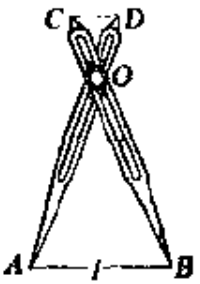
\includegraphics[width=3cm]{../pic/czjh2-ch6-xiti21-06.png}
        \caption*{(第 6 题)}
    \end{minipage}
    \qquad
    \begin{minipage}[b]{4cm}
        \centering
        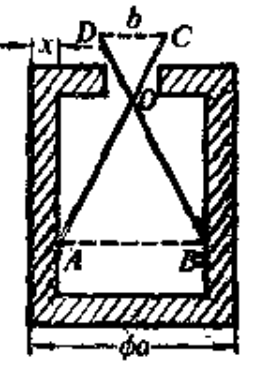
\includegraphics[width=3.5cm]{../pic/czjh2-ch6-xiti21-07.png}
        \caption*{(第 7 题)}
    \end{minipage}
    \qquad
    \begin{minipage}[b]{6cm}
        \centering
        \begin{tikzpicture}
    \tkzDefPoints{0/0/A, 4/0/C, 1.8/0.4/E, 1.8/0/M, 1.8/2.4/D}
    \tkzDefTriangle[two angles=40 and 90](A,C)  \tkzGetPoint{B}
    \tkzDefTriangle[two angles=40 and 50](D,E)  \tkzGetPoint{F}
    \tkzInterLL(D,F)(A,B)  \tkzGetPoint{N}

    \tkzDrawPolygon(A,B,C)
    \tkzDrawPolygon(D,E,F)
    \tkzDrawSegment(E,M)
    \tkzMarkRightAngle(B,C,A)
    \tkzMarkRightAngle(D,F,E)
    \tkzMarkRightAngle(D,M,A)
    \tkzMarkRightAngle(B,N,D)
    \tkzLabelPoints[above](B,D)
    \tkzLabelPoints[left](A)
    \tkzLabelPoints[right](C,F)
    \tkzLabelPoints[above left](E)
\end{tikzpicture}


        \caption*{(第 9 题)}
    \end{minipage}
\end{figure}

\xiaoti{已知如图所示的零件的外径为 $a$,要求它的厚度 $x$,需先求出内孔的直径 $AB$,
    但不能直接量出$AB$。 现用一个交叉卡钳(两条尺长 $AC$ 和 $BD$ 相等)去量,
    若 $\dfrac{OC}{OA} = \dfrac{OD}{OB} = \exdfrac{1}{n}$, 且量得 $CD = b$,
    求厚度 $x$。
}

\xiaoti{证明:}
\begin{xiaoxiaotis}

    \xxt{两个直角三角形有一个锐角相等,两个三角形相似;}

    \xxt{两个等腰三角形的顶角(或底角)相等,两三角形相似;}

    \xxt{两个等腰三角形中,腰和底对应成比例,两个三角形相似。}

\end{xiaoxiaotis}


\xiaoti{如图, $\triangle ABC$ 中, $\angle C$ 为直角;
    $\triangle DEF$ 中, $\angle F$ 为直角;
    $DE \perp AC$, $DF \perp AB$。
    求证: $DF = \dfrac{AC}{AB} \cdot DE$。
}


\xiaoti{已知:四边形 $ABCD$ 中, $AC$ 平分 $\angle DAB$, $\angle ACD = \angle ABC$。
    求证: $AC^2 = AB \cdot AD$。
}

\xiaoti{设 $AD$、$BE$ 和 $CF$ 是 $\triangle ABC$ 的三条高。
    求证: $AD \cdot BC = BE \cdot CA = CF \cdot AB$ (用比例线段证明)。
    (分 $\triangle ABC$ 是锐角三角形、直角三角形和钝角三角形三种情况。)
}

\xiaoti{已知:$\triangle ABC$ 中, $AB = AC$, $\angle A = 36^\circ$,$BD$ 是角平分线。求证:}
\begin{xiaoxiaotis}

    \xxt{$BD = AD$;}
    \xxt{$\triangle ABC \xiangsi \triangle BCD$;}
    \xxt{$BD = \dfrac{\sqrt{5} - 1}{2} AB \approx 0.618 AB$。}

\end{xiaoxiaotis}


\xiaoti{已知:$AD$ 是 $\triangle ABC$ 的角平分线,$BH \perp AD$,垂足为 $H$,
    $CK \perp AD$,垂足为 $K$。求证: $\dfrac{AB}{AC} = \dfrac{DH}{DK}$。
}

\begin{figure}[htbp]
    \centering
    \begin{minipage}[b]{7cm}
        \centering
        \begin{tikzpicture}
    \tkzDefPoints{0/0/B, 4/0/C, 3/3/A}
    \tkzDefLine[bisector](B,A,C)  \tkzGetPoint{d}
    \tkzInterLL(A,d)(B,C)  \tkzGetPoint{D}
    \tkzDefLine[altitude](A,B,D)  \tkzGetPoint{h}
    \tkzInterLL(B,h)(A,D)  \tkzGetPoint{H}
    \tkzDefLine[altitude](A,C,D)  \tkzGetPoint{k}
    \tkzInterLL(C,k)(A,D)  \tkzGetPoint{K}

    \tkzDrawPolygon(A,B,C)
    \tkzDrawSegments(A,H  B,H  C,K)
    \tkzMarkAngles[size=0.4](B,A,D)
    \tkzMarkAngles[size=0.3](D,A,C)
    \tkzMarkRightAngle(C,K,A)
    \tkzMarkRightAngle(A,H,B)
    \tkzLabelPoints[above](A)
    \tkzLabelPoints[left](B,K)
    \tkzLabelPoints[right](C)
    \tkzLabelPoints[below](H)
    \tkzLabelPoints[below right](D)
\end{tikzpicture}


        \caption*{(第 13 题)}
    \end{minipage}
    \qquad
    \begin{minipage}[b]{7cm}
        \centering
        \begin{tikzpicture} % 复杂
    \tkzDefPoints{0/0/B, 4/0/C, 3.6/2/E}
    \tkzDefTriangle[two angles=50 and 60](B,C)  \tkzGetPoint{A} % 设 b、c、a 三个角分别为 50、60、70 度
    \tkzDefTriangle[two angles=25 and 25](A,B)  \tkzGetPoint{D} % 确保角 ADB = 130度(因为 ADE = b = 50 度),其它两个角相加为 50 度即可,不一定非得 25、25 度
    \tkzDefTriangle[two angles=70 and 50](A,D)  \tkzGetPoint{E} % 绘制 ABC 的相似三角形 ADE

    \tkzDrawPolygon(A,B,C)
    \tkzDrawPolygon(A,D,E)
    \tkzDrawSegments(A,D  B,E)
    \tkzLabelPoints[above](A)
    \tkzLabelPoints[left](B)
    \tkzLabelPoints[right](C,E)
    \tkzLabelPoints[below](D)
\end{tikzpicture}


        \caption*{(第 16 题)}
    \end{minipage}
\end{figure}

\xiaoti{已知:$O$ 是 $\triangle ABC$ 内任一点,$OA$、$OB$、$OC$ 的中点分别是 $A'$、$B'$、$C'$。\\
    求证:$\triangle ABC \xiangsi \triangle A'B'C'$。
}

\xiaoti{求证:如果一个三角形的两边和其中一边上的中线与另一个三角形的对应部分成比例,那么这两个三角形相似。}

\xiaoti{已知:如图,$\dfrac{AB}{AD} = \dfrac{BC}{DE} = \dfrac{AC}{AE}$。
    求证:$\angle BAD = \angle CAE$。
}

\xiaoti{求证:如果一个三角形的两边和第三边上的中线与另一个三角形的对应部分成比例,那么这两个三角形相似。}

\xiaoti{如图,在正方形网络上有两个三角形 $A_1B_1C_1$ 和 $A_2B_2C_2$。
    求证: $\triangle A_1B_1C_1 \xiangsi \triangle A_2B_2C_2$。
}

\begin{figure}[htbp]
    \centering
    \begin{minipage}[b]{7cm}
        \centering
        
\begin{tikzpicture}[scale=0.6]
    \pgfmathsetmacro{\a}{6}
    \pgfmathsetmacro{\h}{5}
    \foreach \x in {0,...,\a} {
        \tkzDefPoints{\x/0/X1, \x/\h/X2}
        \tkzDrawSegments(X1,X2)
    }
    \foreach \y in {0,...,\h} {
        \tkzDefPoints{0/\y/Y1, \a/\y/Y2}
        \tkzDrawSegments(Y1,Y2)
    }

    \tkzDefPoints{3/2/A_1, 1/1/B_1, 6/1/C_1}
    \tkzDefPoints{4/3/A_2, 3/4/B_2, 6/3/C_2}
    \tkzDrawPolygon[thick](A_1,B_1,C_1)
    \tkzDrawPolygon[thick](A_2,B_2,C_2)
    \tkzLabelPoints[above left](A_1,B_2)
    \tkzLabelPoints[above,xshift=-.6em](C_2)
    \tkzLabelPoints[below left](B_1,C_1)
    \tkzLabelPoints[below,xshift=-.1em](A_2)
\end{tikzpicture}


        \caption*{(第 18 题)}
    \end{minipage}
    \qquad
    \begin{minipage}[b]{7cm}
        \centering
        \begin{tikzpicture}[scale=.8]
    \tkzDefPoints{0/0/B, 6/0/C, 3/2/A}
    \tkzDefPoints{1/0/D, 2/0/E, 3/0/F, 4/0/G, 5/0/H}
    \foreach \x/\y/\z in {D/M/B, E/N/B, G/K/C, H/L/C} {
        \tkzDefLine[perpendicular=through \x](B,C)  \tkzGetPoint{t}
        \tkzInterLL(\x,t)(A,\z)  \tkzGetPoint{\y}
        \tkzDrawSegment(\x,\y)
        \tkzMarkRightAngle(C,\x,\y)
    }
    \tkzDrawPolygon(A,B,C)
    \tkzDrawSegments(A,F M,E  N,F  K,F  L,G)
    \tkzMarkRightAngle(C,F,A)
    \tkzLabelPoints[above](A,M,N,K,L)
    \tkzLabelPoints[left](B)
    \tkzLabelPoints[right](C)
    \tkzLabelPoints[below](D,E,F,G,H)
\end{tikzpicture}


        \caption*{(第 19 题)}
    \end{minipage}
\end{figure}

\xiaoti{如图,人字形屋架上的六段距离 $BD$、$DE$、$EF$、$FG$、$GH$、$HC$ 彼此相等。
    $MD$、$NE$、$AF$、$KG$、$LH$ 都垂直于 $BC$,中柱 $AF = 2$ 米,求支柱 $DM$、$EN$ 的长度。
}

\xiaoti{求证:如果一个直角三角形的一条直角边和斜边上的高,与另一个直角三角形的一条直角边和斜边上的高成比例,
    那么这两个三角形相似。
}

\end{enhancedline}
\end{xiaotis}

